\subsection{Problem and Motivations}

\noLogo{
\begin{frame} \frametitle{Problem and Motivations}

{
\setbeamercovered{invisible}
\begin{itemize}

\item<1-> Network graph G(V,E): V = modules, E = connections\\
\begin{itemize}
	\item<1-> Neighbor-to-Neighbor communications, unique node identifiers
	\item<1-> $d(v_i, v_j)$ = hop distance between modules $v_i$ and $v_j$
\end{itemize}

\item<2-> Problem: efficient election of an approximate central node

\item<3-> Central nodes?
\begin{itemize}

\item<4-> Center: minimizes the maximum distance to all the others\\
\hspace{2cm}$Center = \argmin\limits_{v_i \in V} ecc (v_i) = \argmin\limits_{v_i \in V} \max\limits_{v_j \in V} d(v_i,v_j)$

\item<5-> Centroid: minimizes the average distance to all the others\\
\hspace{2cm}$Centroid = \argmin\limits_{v_i \in V} \frac{1}{|V|} \sum\limits_{v_j \in V} d(v_i,v_j)$ 

%\item Betweenness center: nodes on most shortest-paths
\end{itemize}

\item<6-> Challenge: requires a distributed all-pair shortest path computation
	\begin{itemize}
		\item Large time, message and/or storage costs.	
	\end{itemize}

\item<7-> Motivation: ideal nodes for communications with all the others
	\begin{itemize}
		\item Example: service providers
			\begin{itemize}
				\item Time synchronization: the precision decreases with the hop distance to the time master
			\end{itemize}
	\end{itemize}
\end{itemize}
}

\only<1-3>{
	\begin{textblock*}{\paperwidth}(-0.5cm,0.57\paperheight)
		\begin{figure}
	  		\centering
	  		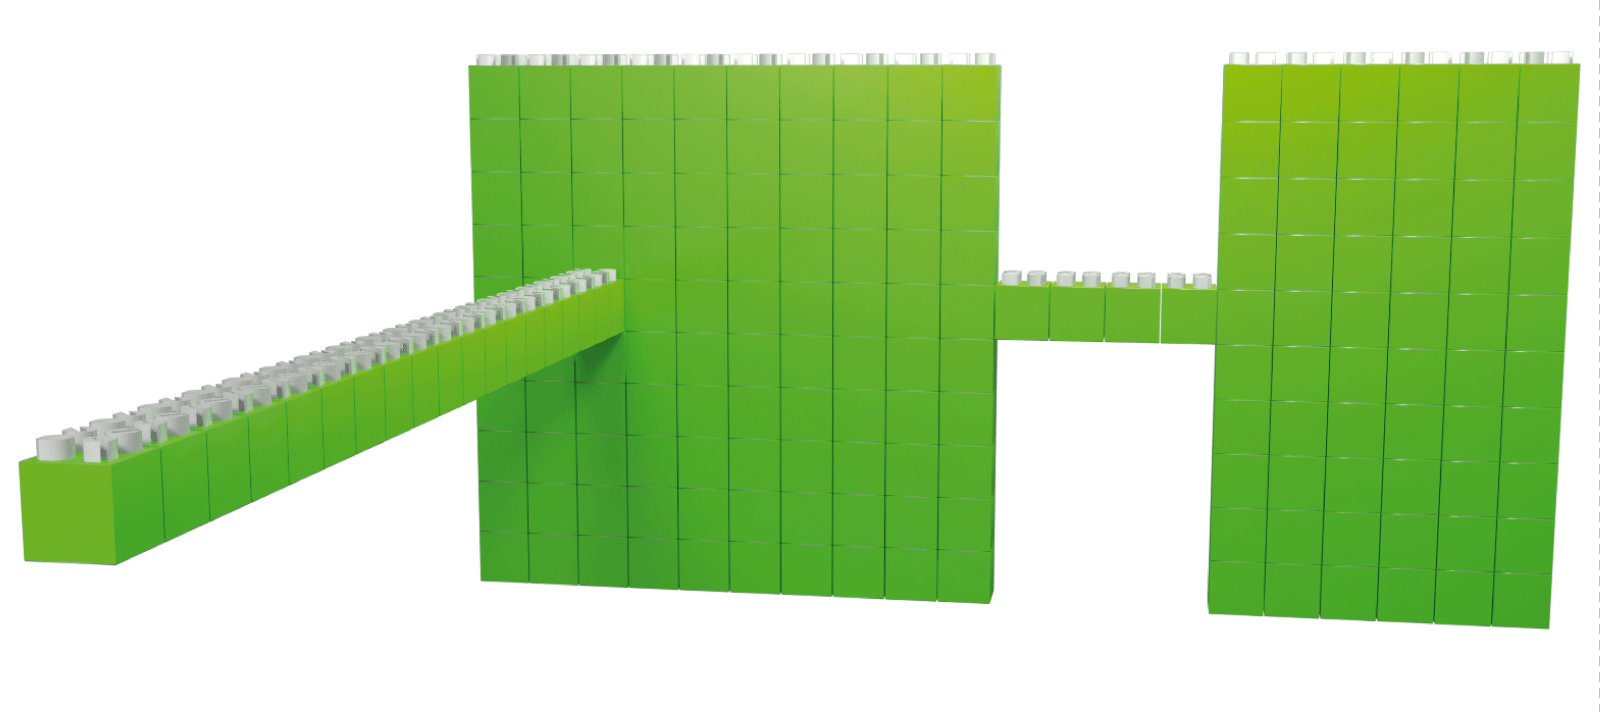
\includegraphics[height=0.35\paperheight]{fig/centrality/centers/initial}
	  	\end{figure}
	\end{textblock*}
}

\only<4>{
	\begin{textblock*}{\paperwidth}(-0.5cm,0.57\paperheight)
		\begin{figure}
			\centering
			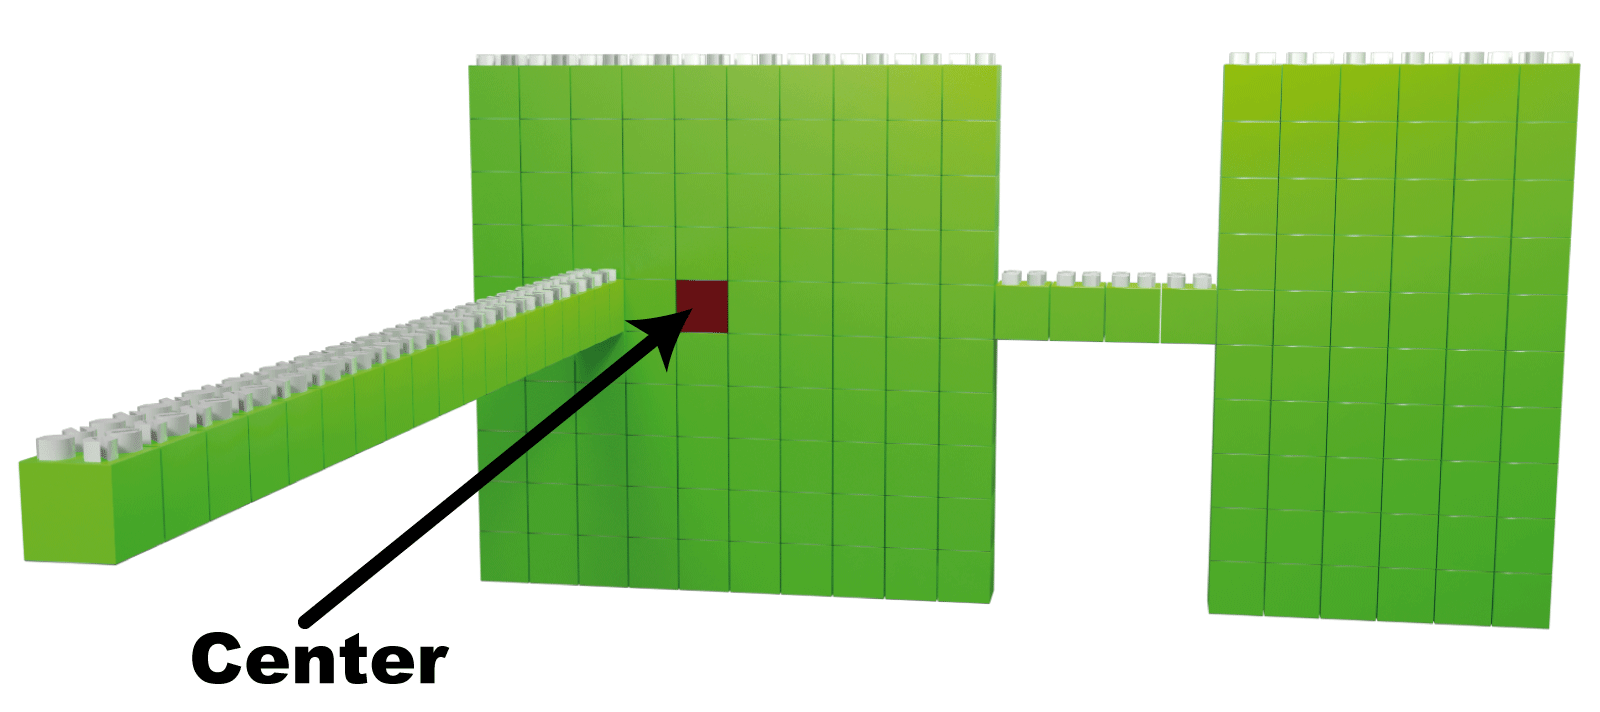
\includegraphics[height=0.35\paperheight]{fig/centrality/centers/center}
		\end{figure}
	\end{textblock*}
}

\only<5>{
	\begin{textblock*}{\paperwidth}(-0.5cm,0.57\paperheight)
		\begin{figure}
			\centering
			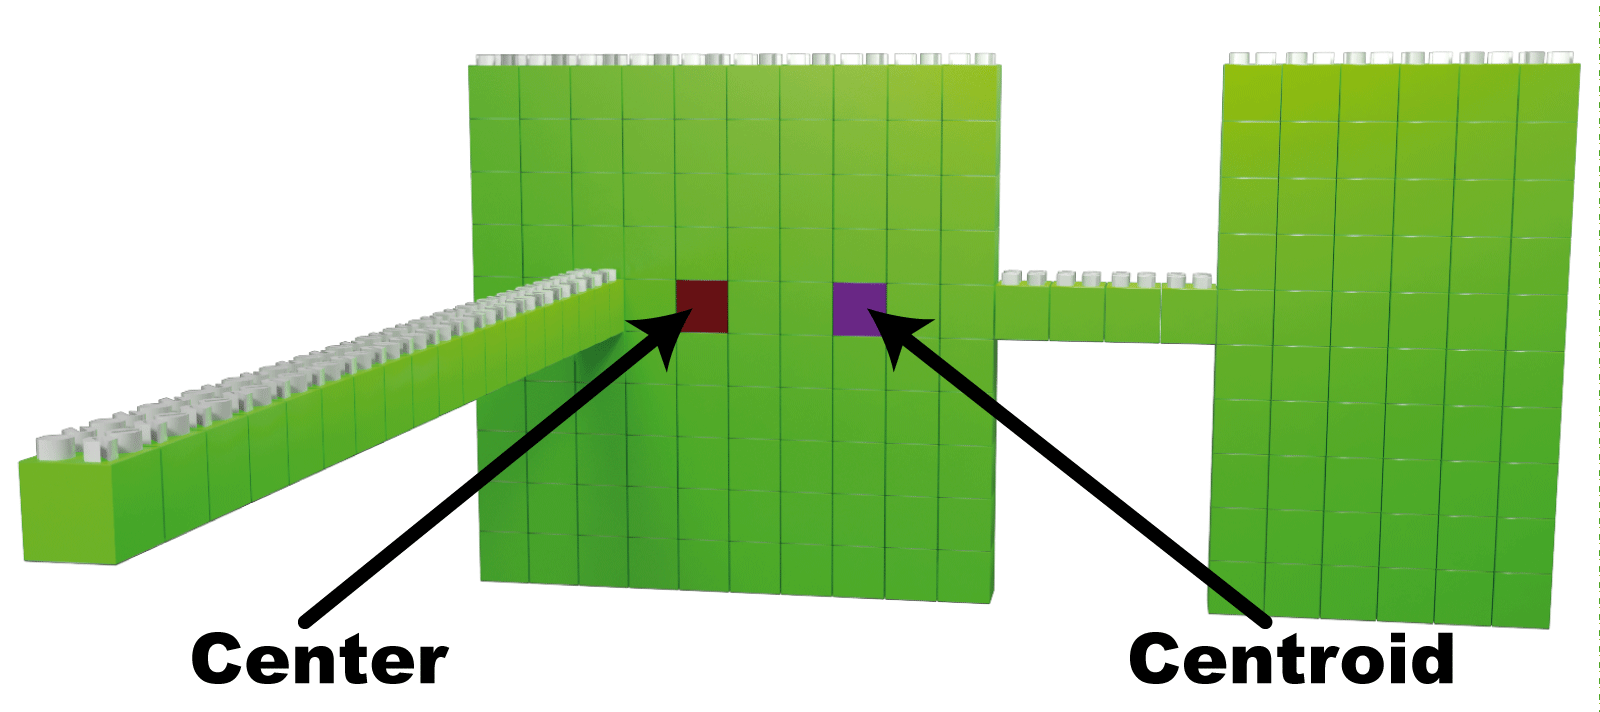
\includegraphics[height=0.35\paperheight]{fig/centrality/centers/center-centroid}
		\end{figure}
	\end{textblock*}
}

\end{frame}
}

\subsection{Related Work and Contributions}

\subsectionOutlineFrame

\noLogo{
\begin{frame} \frametitle{Related Work}
%TM vs decentralized
%clock skew compensation
{
	\footnotesize
	
	\newcommand{\lenTwo}{0.17\linewidth}
	\newcommand{\lenThree}{0.32\linewidth}
	\newcommand{\lenFour}{0.3\linewidth}

	\begin{center}
		\begin{tabular}{|C{\lenThree}|C{\lenTwo}|C{\lenTwo}|C{\lenTwo}|}
			\hline
			Approach & Accuracy (experiments) & Time and message cost & Memory cost\\ 
			\hline
			Naive and exhaustive (e.g., \cite{Korach:1984:DAF:579.585,mamei2005self}) & exact & +++++\hspace{2cm} (potential congestion) & + to +++++
			 \\
			\hline
			Graph specific (e.g., \cite{bruell1999self} for trees) & exact (but not for arbitrary graphs) & + & +\\
			\hline
			Approximation (e.g., \cite{wehmuth2013daccer, dissler2016distributed, kim2013leader}) & ++ to +++ & ++ & + to +++\\
			\hline
		\end{tabular}
	\end{center}

	Thesis contribution: %approximation algorithms for arbitrary networks
	\begin{center}
		\begin{tabular}{|C{\lenThree}|C{\lenTwo}|C{\lenTwo}|C{\lenTwo}|}
			\hline
			3 approximation algorithms & +++ to ++++ & +++ & + \\
			%(inspired from external- graph analysis methods)
			\hline
		\end{tabular}
	
	\remark{A good cost-accuracy trade-off}
	\end{center}


}

\end{frame}
}

\begin{frame} \frametitle{My Contributions}

\begin{itemize}
	\item 3 distributed algorithms:
	\begin{itemize}
		\item $k$-BFS SumSweep
		\item { ABC-Center} (two versions) %\bfseries
		\item Probabilistic Counter based Central Leader Election (PC2LE)
	\end{itemize}
	\item Inspired from existing external-graph analysis algorithms
	\item All based on intuitive heuristics
	\item Experimental evaluation of the accuracy
	\item Formal analysis of the performance:

{
	\scriptsize
	\newcommand{\lenOne}{0.12\linewidth}
	\newcommand{\lenFive}{0.17\linewidth}

\begin{center}
	\begin{tabular}{|C{\lenFive}|C{\lenOne}|C{\lenFive}|C{\lenFive}|C{\lenFive}|}
		\hline
		Name & Type of center & Time & Memory (per module) & Message\\
		\hline
		$k$-BFS SumSweep & center, centroid & $O(k\times d)$ & $O(\Delta)$ & $O(m \times n^2)$ \\
		\hline
		ABC-CenterV2 & center & O($\#steps \times d$) & $O(\Delta)$ & $O(m \times n^2)$ \\
		\hline
		PC2LE & center, centroid & O($d$) & $O(\Delta + $ $|$probabilistic counter$|)$ & $O(m \times n^2)$ \\
		\hline
	\end{tabular}
\end{center}
	Notation:\\
	$n = \# $modules, $m = \#$ links, $d = $ diameter, $\Delta = $ maximum number of neighbors\par
}
\end{itemize}

\end{frame}

\subsection{ABC-CenterV2}

\subsectionOutlineFrame

\subsubsection{General Idea}

\begin{frame} \frametitle{General Idea}

\begin{itemize}
	\item Extends the sequential MiniMax algorithm~\cite{handler1973minimax} for tree graphs
	\item Idea: the center stands at the middle of a diameter (i.e., longest path)
\end{itemize}

\begin{center}
	\begin{columns}[c]
	\begin{column}{.5\textwidth}
		\centering
		\adjincludegraphics[width=1\linewidth,valign=c]{fig/centrality/abc-centerv2/mid-diameter-4.png}
	\end{column}
	\begin{column}{.3\textwidth}
		\only<2> {
			\centering
			\adjincludegraphics[width=\linewidth,valign=c]{fig/centrality/twoSweep.png}
		}
	\end{column}
\end{columns}
\end{center}

\end{frame}

\subsubsection{Algorithm}

\begin{frame} \frametitle{Algorithm}

\begin{center}
\myAlg{
	{$Candidates\gets all\ modules$\;}
	
	\While{$|Candidates| > 2$}{
		
		{$A \gets v_i \in Candidates$;\ \tcp{A is a random candidate}}
		
		{$B \gets v_i \in \argmax\limits_{v_j \in Candidates} d(A, v_j)$;\ \tcp{B a farthest candidate from A}}
		
		{$C \gets v_i \in \argmax\limits_{v_j \in Candidates} d(B, v_j)$;\ \tcp{C a farthest candidate from B}}
				
		\tcp{Most equi-distant nodes from B to C remain candidate:}
		{$Candidates \gets  \argmin\limits_{v_j \in Candidates} |d(B,v_j) - d(C,v_j)| $\;}
	
		\tcp{\footnotesize B and C are eliminated (if not already purged by the previous line):}
		{$Candidates \gets Candidates - \{B, C\}$\;}
	}
	
	{$central \gets  v_i \in Candidates$;\ \tcp{a random candidate}}
}
\end{center}

Single-source shortest paths are computed using distributed breadth-first network traversals (based on~\cite{cheung1983graph}).

\end{frame}

\subsubsection{Examples}

\begin{frame} \frametitle{Examples - One-step 2D Shape}

\only<1> {
	\begin{figure}
		\centering
		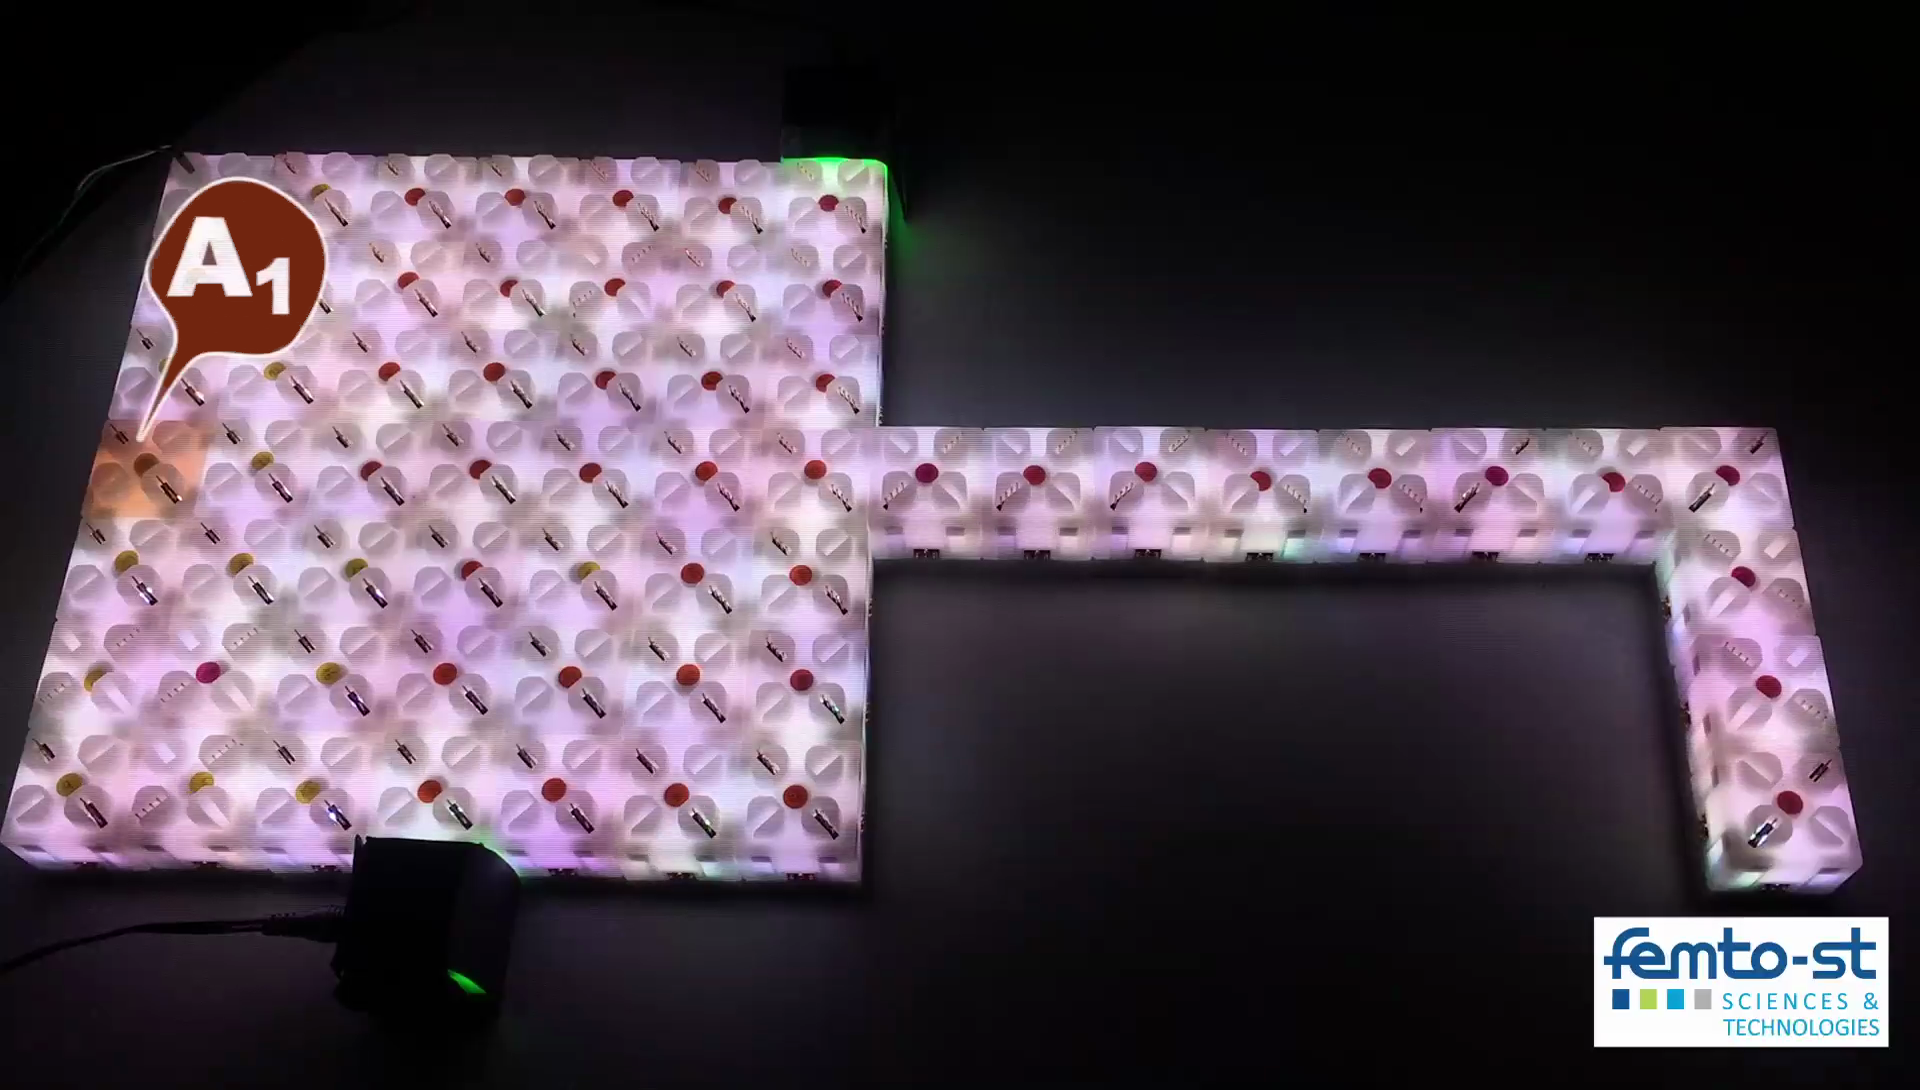
\includegraphics[width=0.7\linewidth]{fig/centrality/abc-center-example-2/1}
	\end{figure}
}

\only<2> {
	\begin{figure}
		\centering
		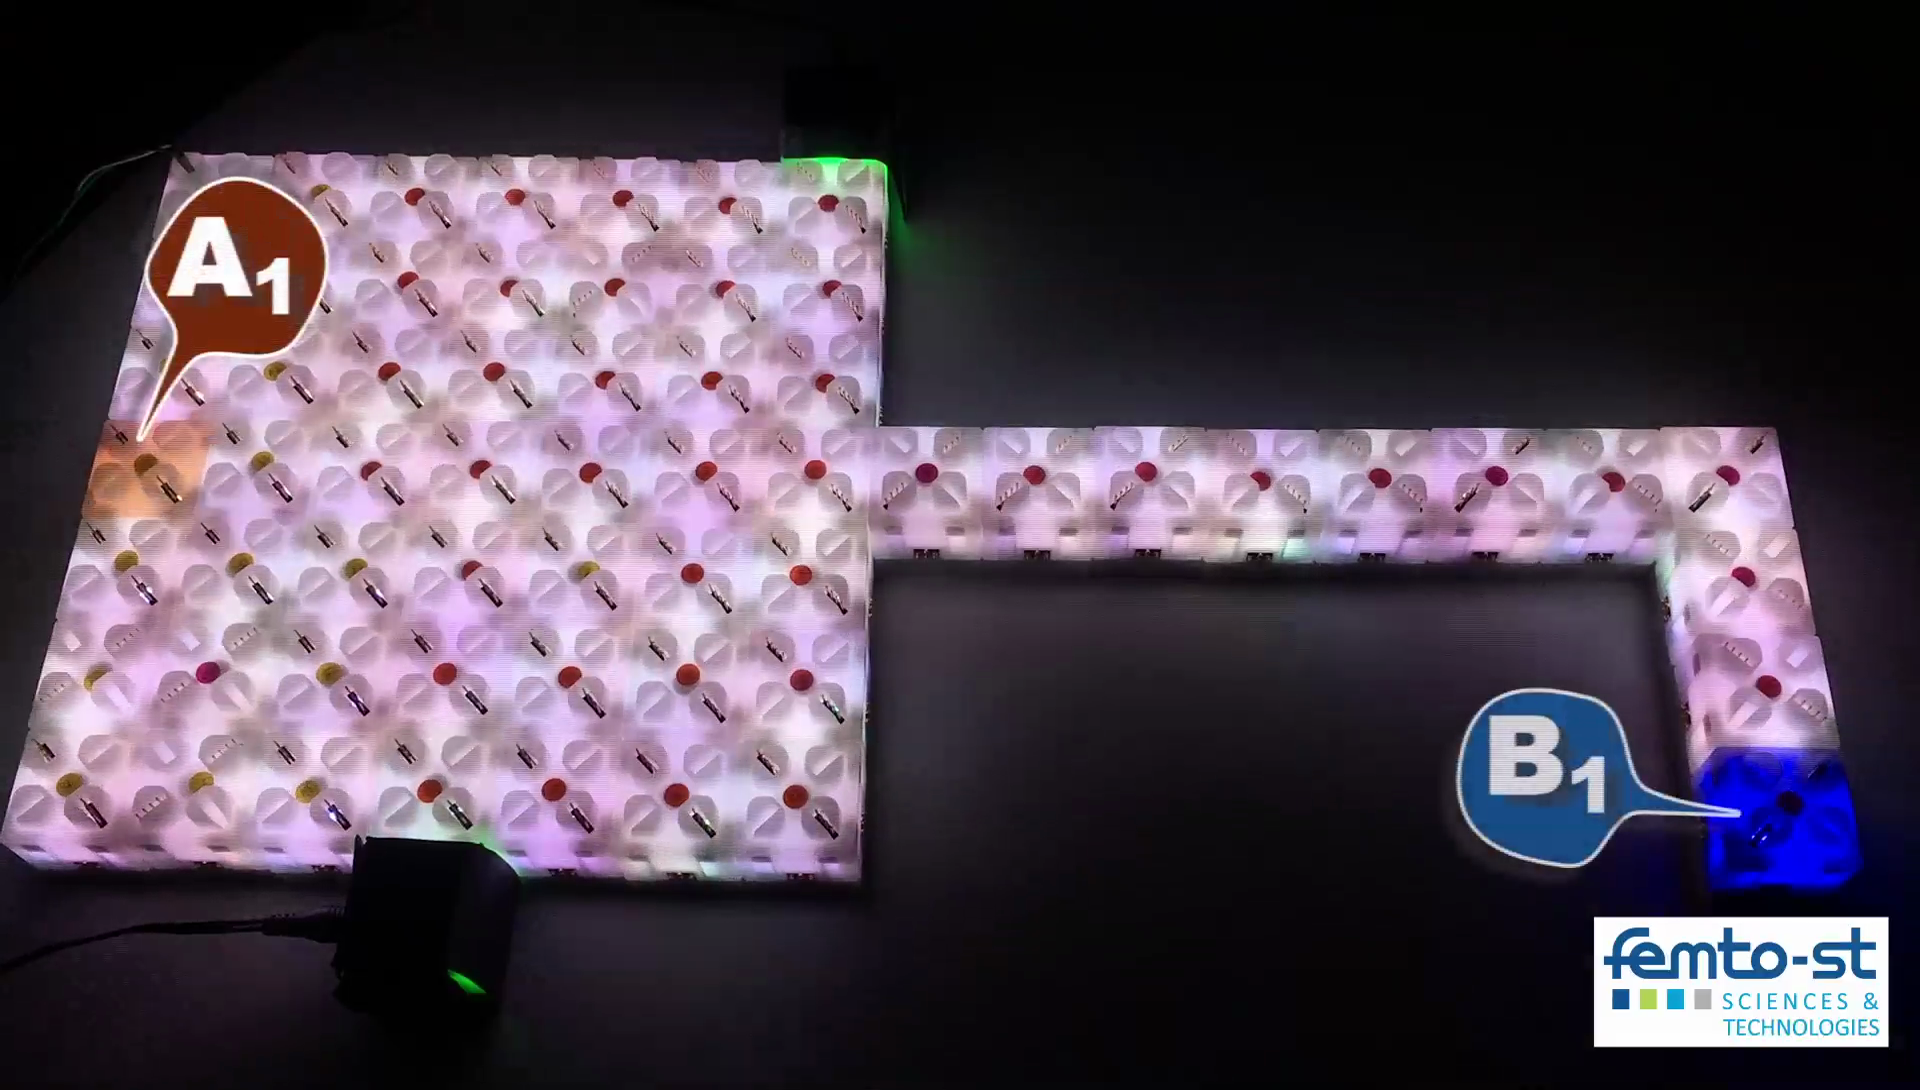
\includegraphics[width=0.7\linewidth]{fig/centrality/abc-center-example-2/2}
	\end{figure}
}

\only<3> {
	\begin{figure}
		\centering
		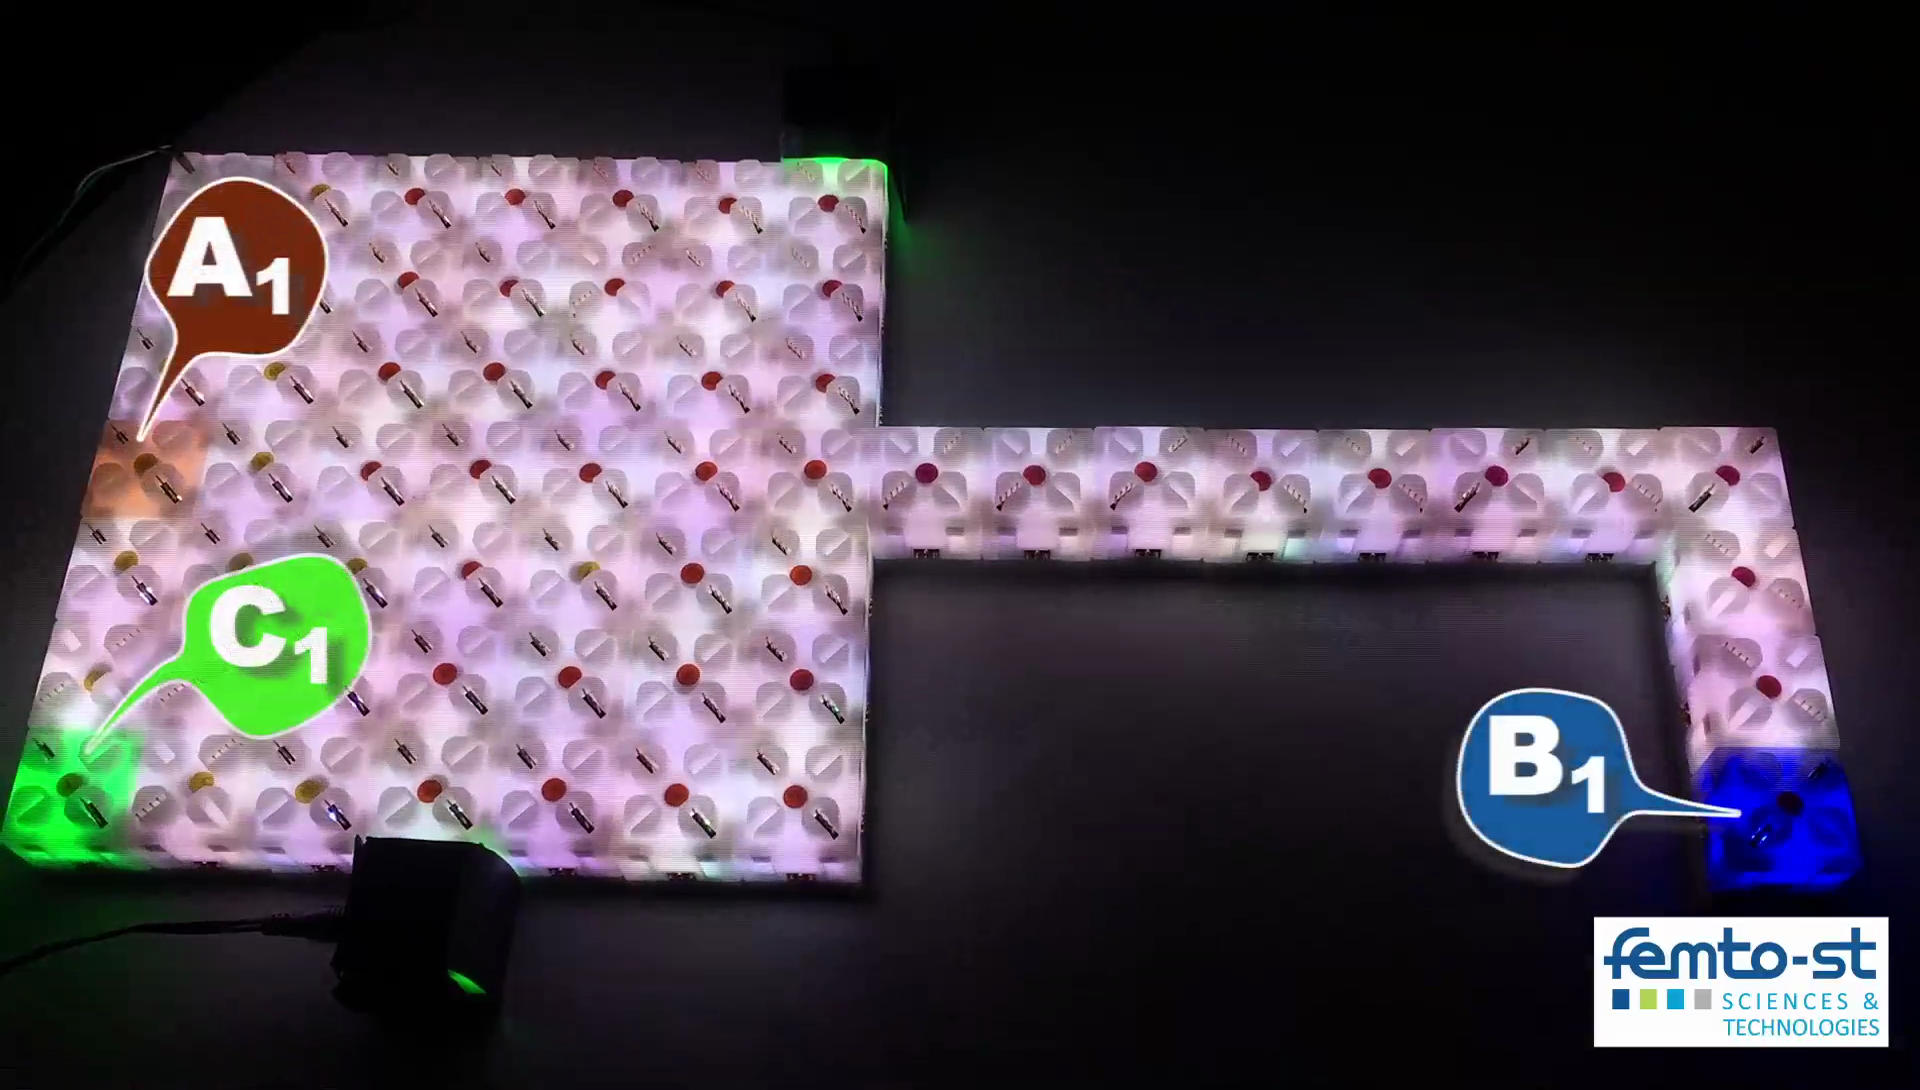
\includegraphics[width=0.7\linewidth]{fig/centrality/abc-center-example-2/3}
	\end{figure}
}

\only<4> {
	\begin{figure}
		\centering
		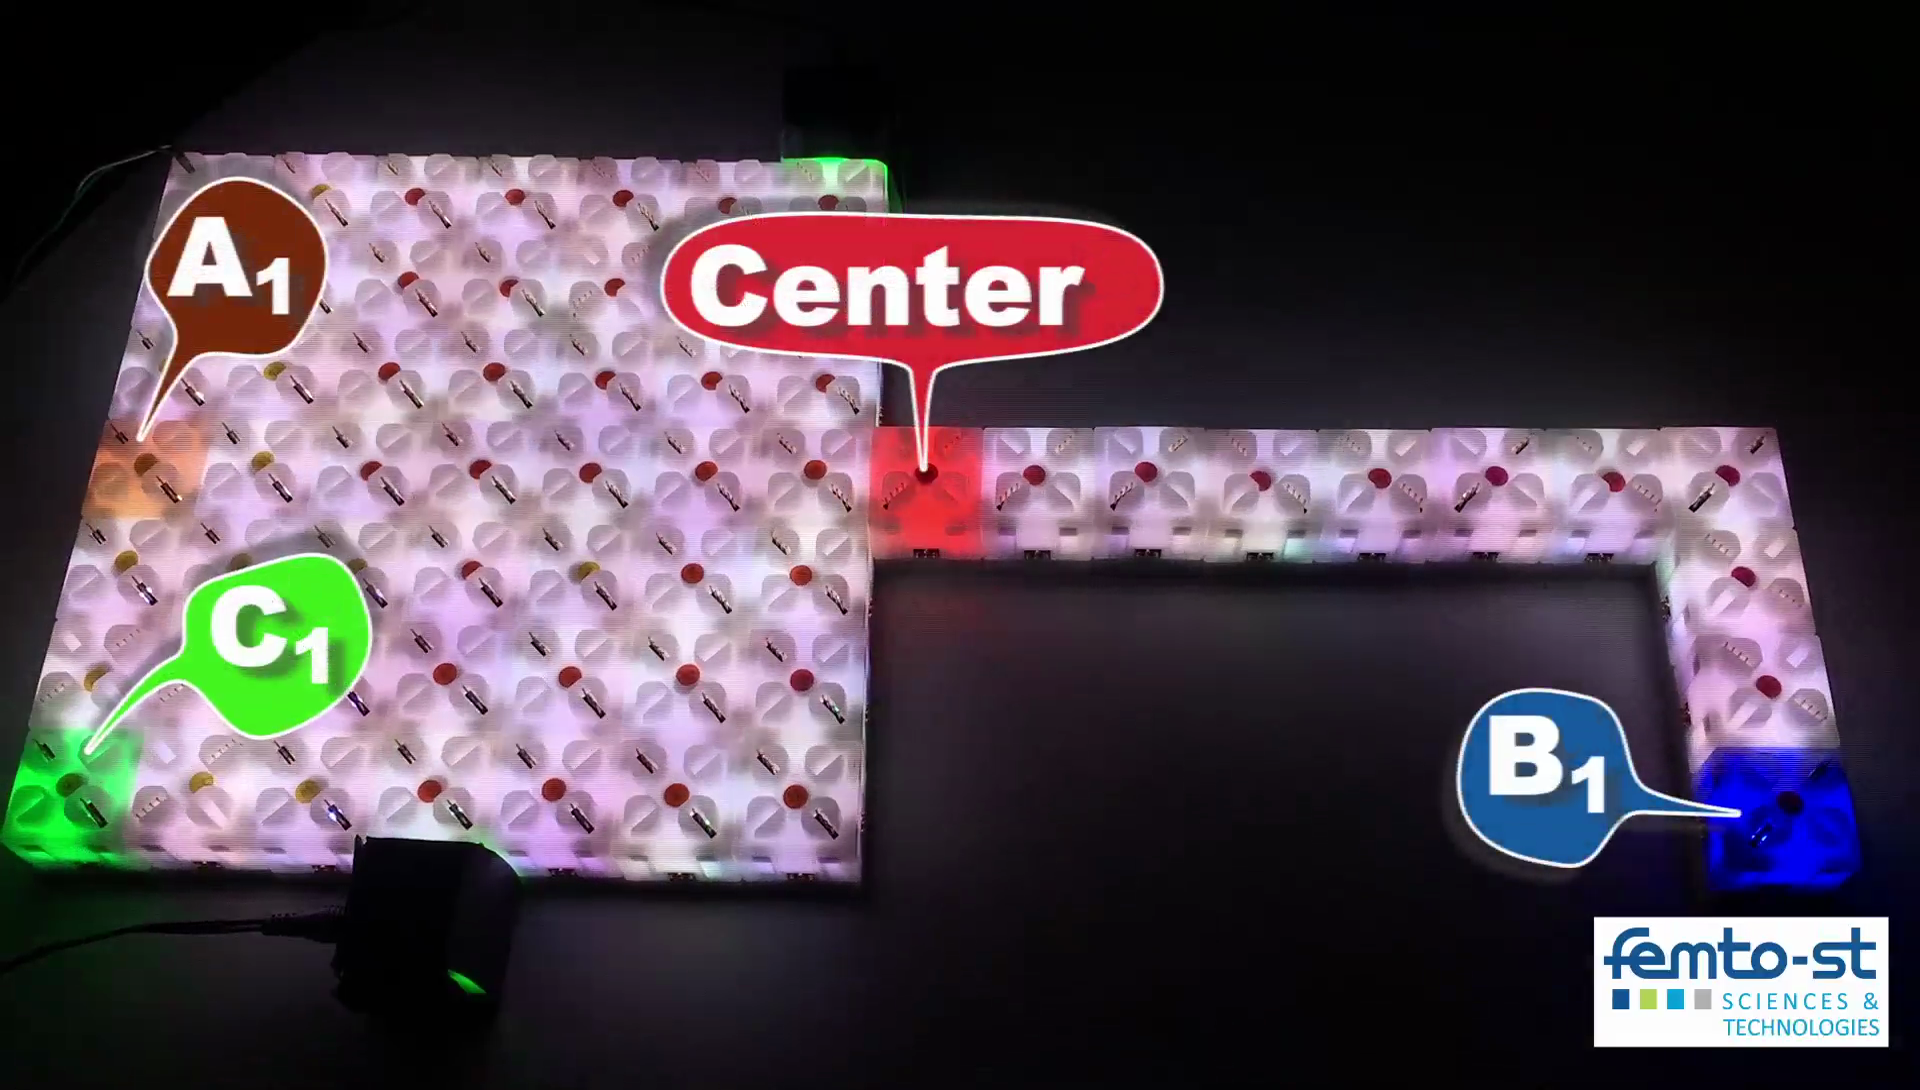
\includegraphics[width=0.7\linewidth]{fig/centrality/abc-center-example-2/4}
	\end{figure}
}

\begin{center}
	\vspace{-0.5cm}\hspace*{5cm}$^*$60 Blinky Blocks
\end{center}

\end{frame}

\begin{frame} \frametitle{Examples - More complex}
\vspace{1cm}
\begin{center}
\only<1> {
	\begin{figure}
		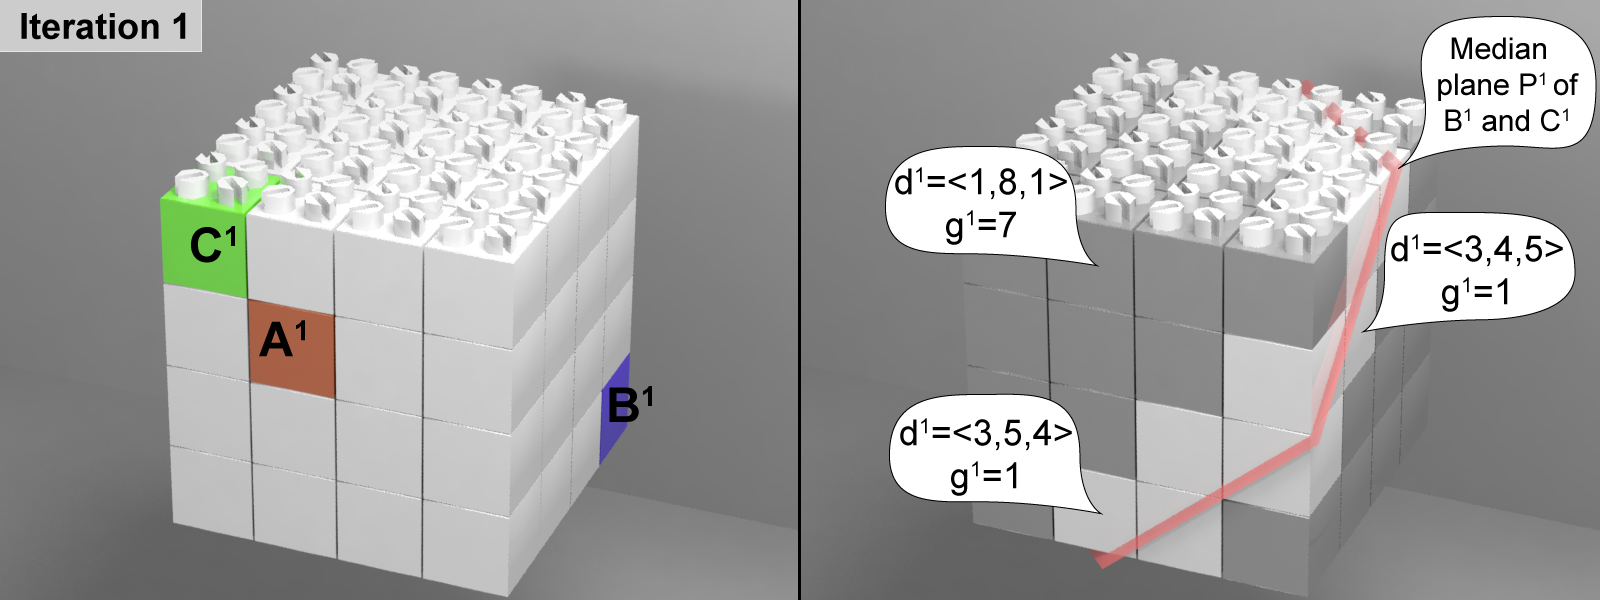
\includegraphics[width=\linewidth]{fig/centrality/abc-centerv2/cube/step1}
	\end{figure}
}

\only<2> {
	\begin{figure}
		\centering
		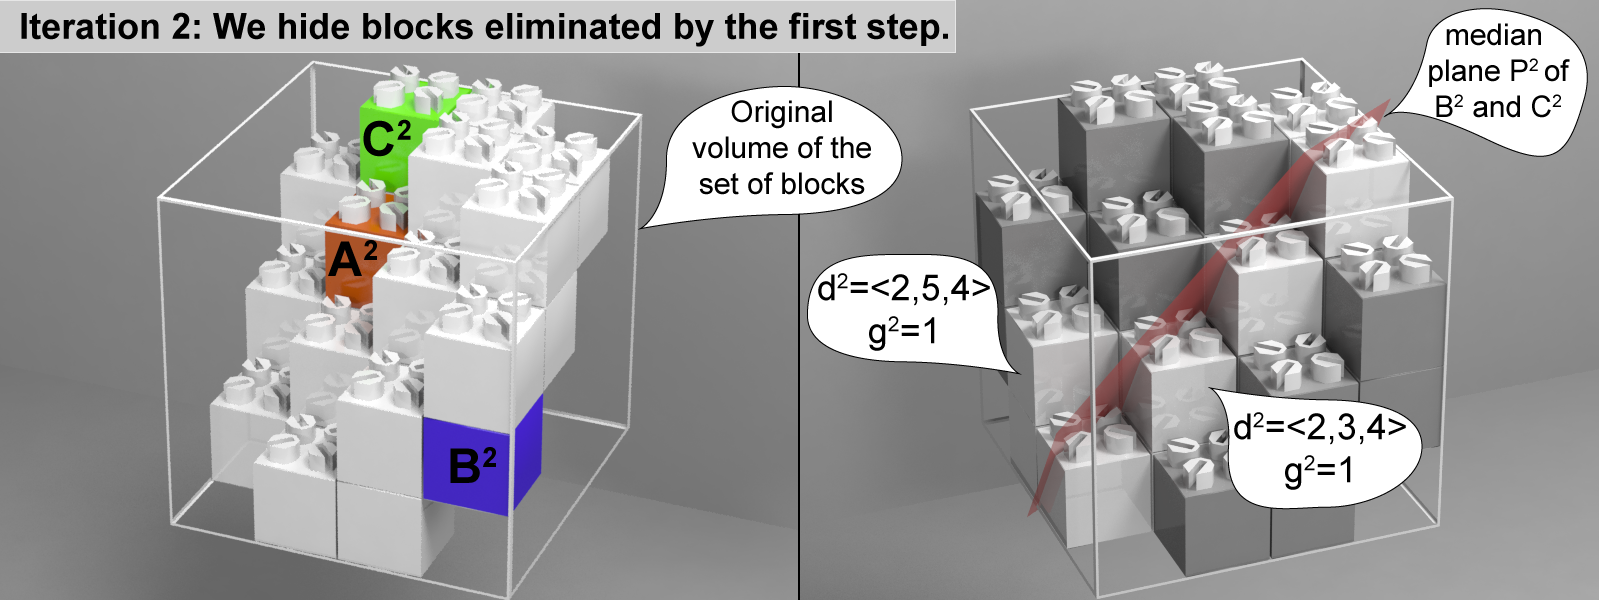
\includegraphics[width=\linewidth]{fig/centrality/abc-centerv2/cube/step2}
	\end{figure}
}

\only<3> {
	\begin{figure}
	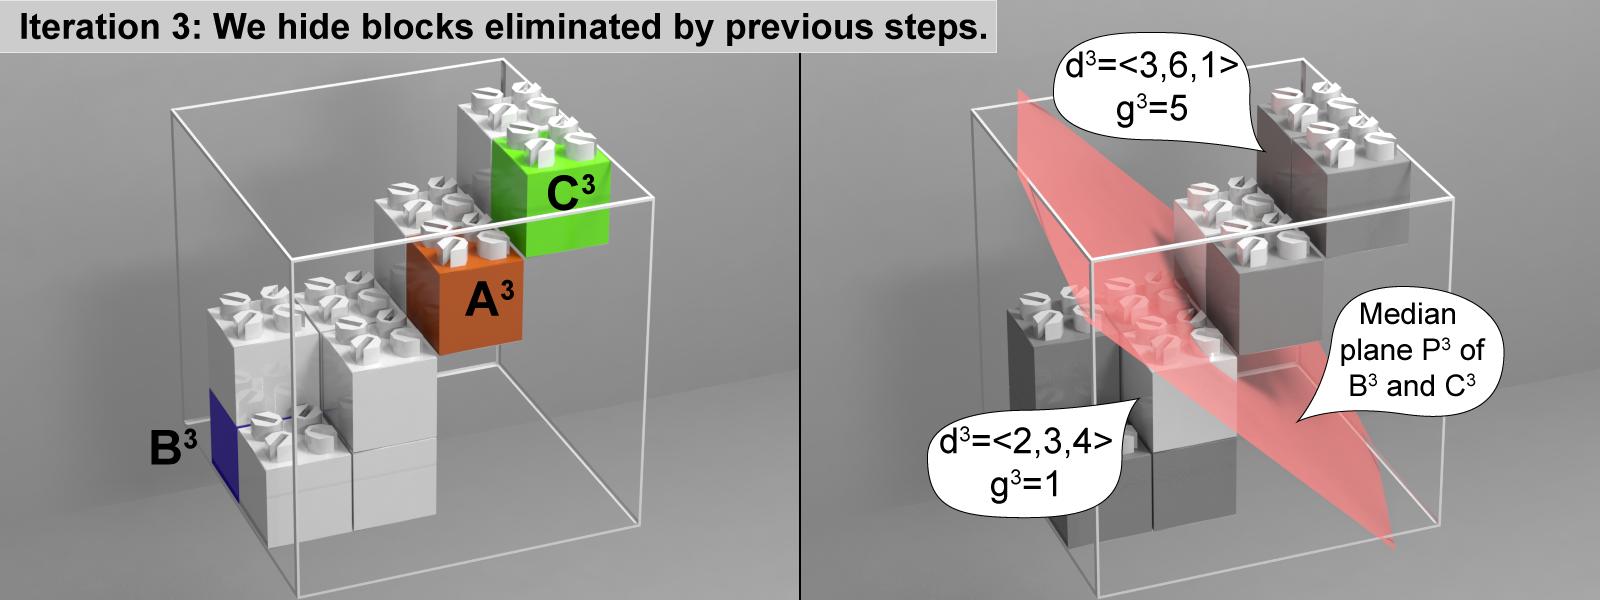
\includegraphics[width=\linewidth]{fig/centrality/abc-centerv2/cube/step3}
	\end{figure}
}

\only<4-> {
	\begin{figure}
		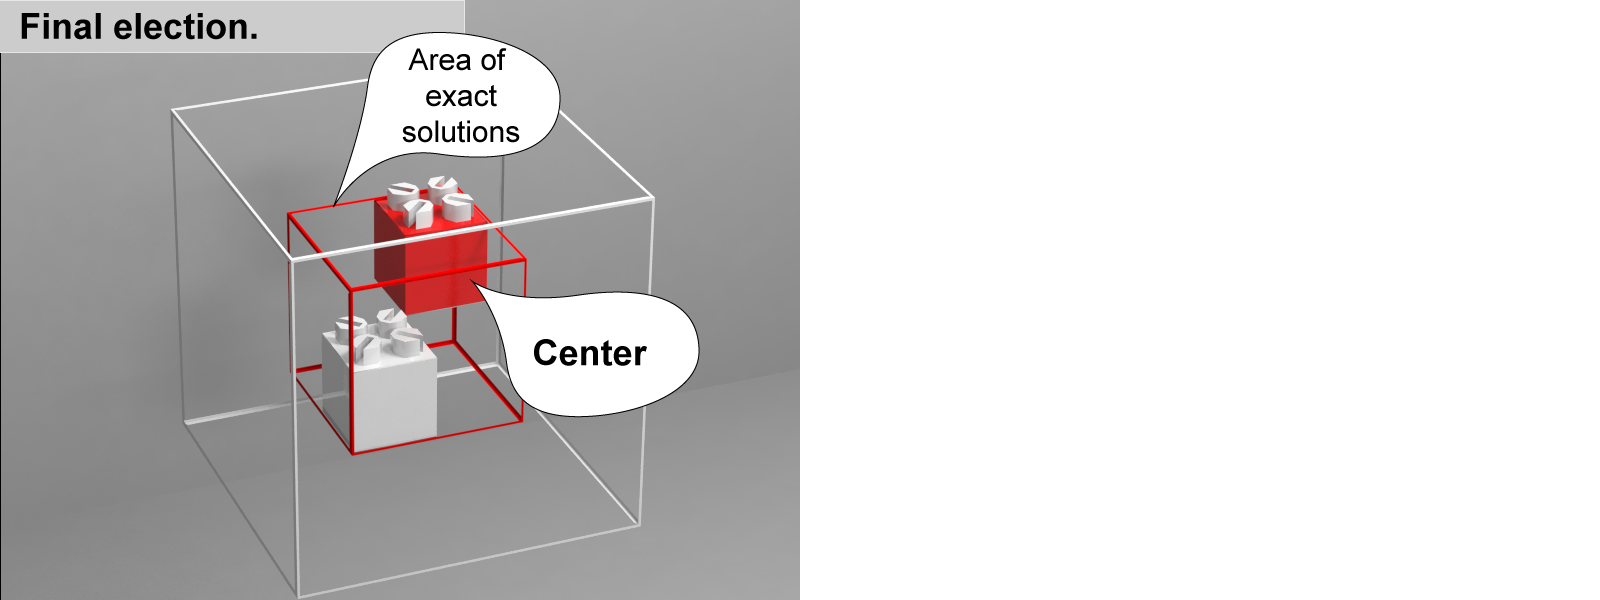
\includegraphics[width=\linewidth]{fig/centrality/abc-centerv2/cube/step4}
	\end{figure}
}
\end{center}

\only<5>{
	\remark{$\#$ steps increases with the thickness of the diameter}
	\remark{ABC-Center is more efficient in low-degree networks}
}
\end{frame}

\subsubsection{Tricky Case}

\begin{frame} \frametitle{Tricky Case for Future Work}
\begin{center}
	\begin{columns}[T]
		\begin{column}{.45\textwidth}
			\centering
			\adjincludegraphics[width=\linewidth]{fig/centrality/tricky-case/abc-center.png}
			ABC-CenterV1/V2
		\end{column}
		\begin{column}{.45\textwidth}
			\only<2-> {
				\centering
				\adjincludegraphics[width=\linewidth]{fig/centrality/tricky-case/trial.png}
				Envisioned but abandoned approach
			}
		\end{column}
	\end{columns}

\only<3> {
	\vspace*{0.5cm}
\remark{The envisioned approach solves this case but leads to less accuracy in experiments with random systems}

\remark{This specific case should be investigated in future work!}
}

\end{center}
\end{frame}

\subsection{Evaluation}

\subsectionOutlineFrame

\subsubsection{ABC-CenterV1 on Hardware}

\noLogo{
\begin{frame} \frametitle{ABC-CenterV1 on Hardware}

	\begin{figure}
	\centering
	\href{run:videos/21-abccenter-dynamics.avi?autostart&loop}{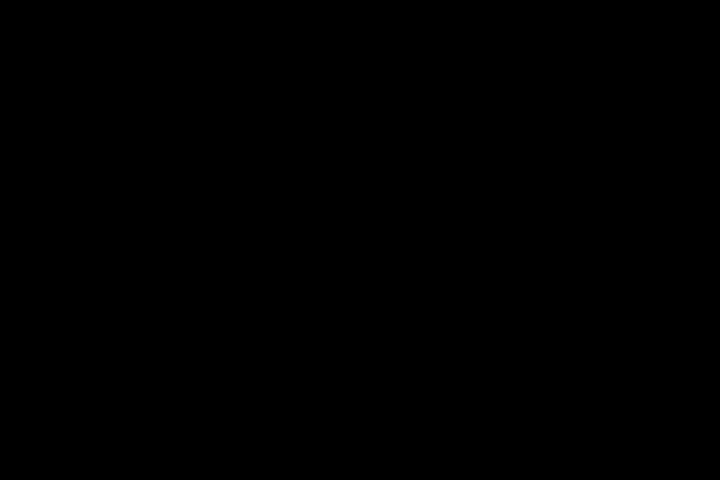
\includegraphics[width=0.7\textwidth]{videos/21-abccenter-dynamics.jpg}}
	\end{figure}

\end{frame}
}

\subsubsection{Simulation Fidelity}

\noLogo{
\begin{frame} \frametitle{VisibleSim Simulator Fidelity}

Statistical simulation model based on measurements
\begin{itemize}	
	\item Processing time
	\item Communication time
\end{itemize}

	{
		
		\newcommand{\vsfid}[1]{rien}
		\newcommand{\lenOneOne}{0.07\linewidth}
		\newcommand{\lenTwoTwo}{0.12\linewidth}
		\newcommand{\lenThreeThree}{0.15\linewidth}
		\newcommand{\lenFourFour}{0.2\linewidth}
		\begin{table}[!h]
			\centering			
			\small
			\begin{tabular}{|C{\lenTwoTwo}|C{\lenTwoTwo}|C{\lenThreeThree}|C{\lenThreeThree}|C{\lenFourFour}|}
				\hline
				& & \multicolumn{2}{c|}{average ABC-CenterV1} &  \\
				Shape & Size & \multicolumn{2}{c|}{execution time} &  \textcolor{\remarkColor}{Relative average}   \\
				 &  (module) & \multicolumn{2}{c|}{$\pm$ standard-deviation (ms)}& \textcolor{\remarkColor}{simulation} \\
				\cline{3-4}
				&  & Hardware & Simulator & \textcolor{\remarkColor}{precision}\\
				\hline
				\multirow{3}{*}{Line}  & 5 & $234 \pm 1$ & $244 \pm 3$ & \textcolor{\remarkColor}{95.7\%} \\
				%529611
				\cline{2-5}
				& 10 & $545 \pm 5$ & $544 \pm 5$ & \textcolor{\remarkColor}{99.8\%}\\
				%529611
				\cline{2-5}
				& 50 & $2873 \pm 23$ & $2885 \pm 17$ & \textcolor{\remarkColor}{99.6\%}\\
				%2879659
				\hline
				\multirow{3}{*}{Square} & 9 & $598 \pm 45$ & $588 \pm 14$ & \textcolor{\remarkColor}{98.3\%}\\
				\cline{2-5}
				& 25 & $1117 \pm 30$ & $1119 \pm 27$ & \textcolor{\remarkColor}{99.8\%}\\
				\cline{2-5}
				& 49 & $1684 \pm 48$ & $1686 \pm 44$ & \textcolor{\remarkColor}{99.9\%} \\
				% sim: 1646128
				\hline
				\multirow{2}{*}{Cube} & 27 &$ 1229 \pm 56$ & $ 1214 \pm 31$ & \textcolor{\remarkColor}{98.8\%} \\
				\cline{2-5}
				& 64 & $1927 \pm 51$ & $1941 \pm 33$ & \textcolor{\remarkColor}{99.3\%} \\
				\hline
				Dumbbell & 59 & $1262 \pm 56$ & $1252 \pm 57$& \textcolor{\remarkColor}{99.2\%} \\
				\hline
			\end{tabular}
		\end{table}
	}

\remark{VisibleSim accurately simulates our algorithm on the Blinky Blocks}
	
\end{frame}
}

\subsubsection{Simulation Evaluation}

\newcommand{\ResultsScaleFactor}{1}

\begin{frame} \frametitle{Simulation Evaluation}

\begin{itemize}
	\item Simulations using VisibleSim
	\item Comparisons with other algorithms
	\begin{itemize}
		\item Random: MIN-ID~\cite{raynal2013distributed}
		\item Exhaustive: BARYCENTER~\cite{mamei2005self}
		\item Approximations:
		\begin{itemize}
			\item  TBCE~\cite{kim2013leader}
			\item  $k$-BFS-RAND, our distributed version of~\cite{eppstein2001fast}
			\item PC2LE with \cite{garin2012distributed} 's probabilistic counter
		\end{itemize}
	\end{itemize}
	\item Systems
	\begin{itemize}
		\item Random compact shapes
		%: randomly connecting\\modules one-by-one starting from a\\ single module.
		\item Different sizes: 10 to 25,000 modules
		\item Statistics on multiple independent\\runs
	\end{itemize}
	\item Evaluation criteria
	\begin{itemize}
		\item Accuracy
		\item Cost
		\begin{itemize}
			\item Execution time
			\item Number of messages
			\item Memory usage
		\end{itemize}
	\end{itemize}
	\end{itemize}

\begin{textblock*}{0.39\paperwidth}(0.6\paperwidth,0.45\paperheight)
	
	\begin{figure}
		\centering
		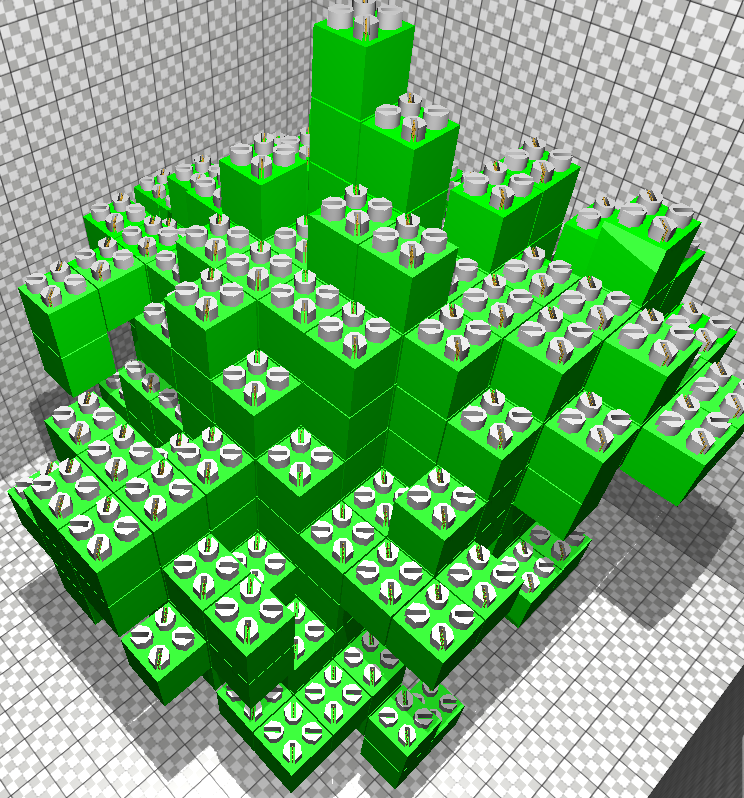
\includegraphics[width=0.8\linewidth]{fig/centrality/random-500modules}
	\end{figure}
\end{textblock*}
\end{frame}

\noLogo{
\begin{frame} \frametitle{Relative accuracy}

{
	\small
	\begin{align*}
	relative\ center\ accuracy = 1 - \left|\frac{ecc(center)- ecc(elected\ node)}{ecc(center)}\right|
	\end{align*}
}
\vspace{-0.25cm}
\begin{figure}
	\centering
	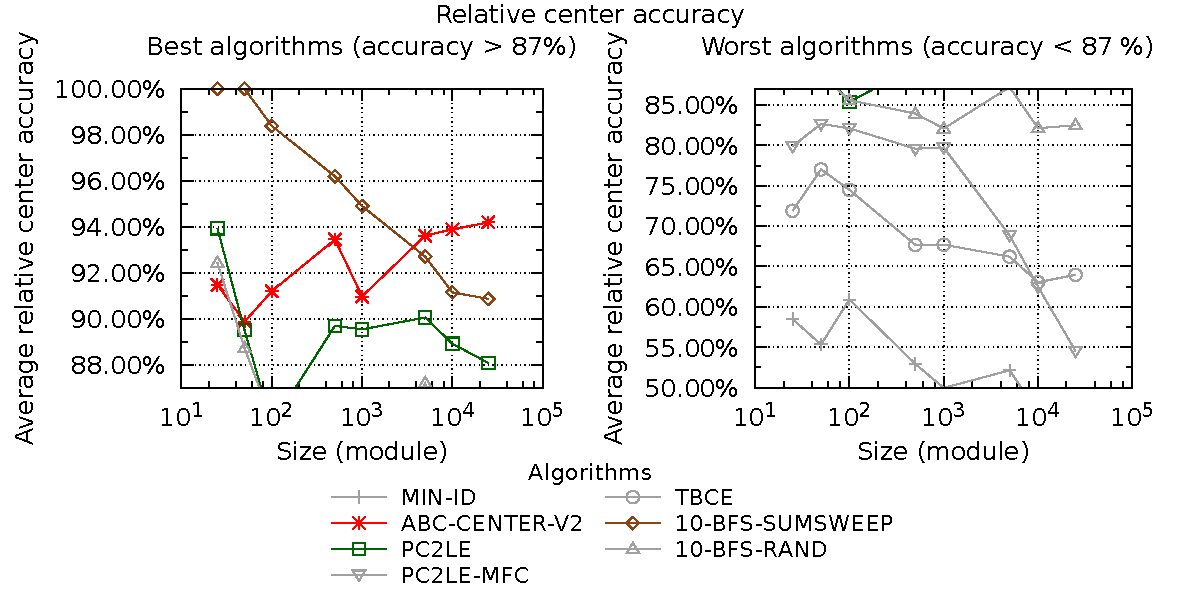
\includegraphics[width=0.825\linewidth]{fig/centrality/accuracy-center}
\end{figure}

\remark{Our algorithms:\\most precise approximation algorithms (accuracy $> 85\%$)}

\end{frame}
}

\begin{frame} \frametitle{Execution Time}

\begin{center}
	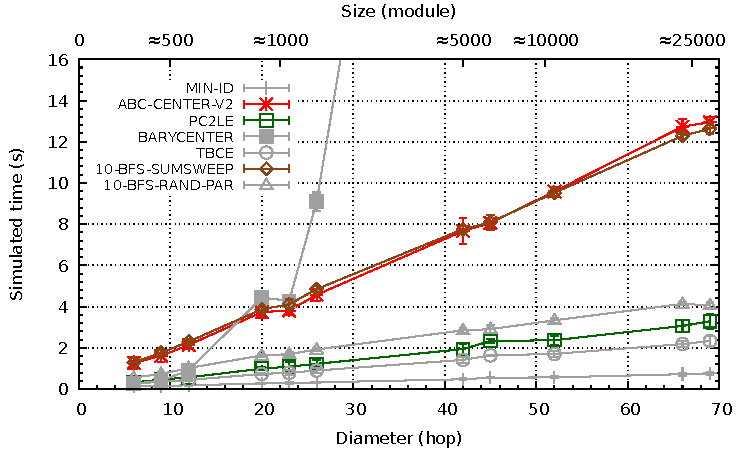
\includegraphics[width=0.9\linewidth]{fig/centrality/time}
\end{center}
\remark{A good trade-off between cost and accuracy}
\end{frame}


\begin{frame} \frametitle{Average number of messages per module}
\begin{center}
	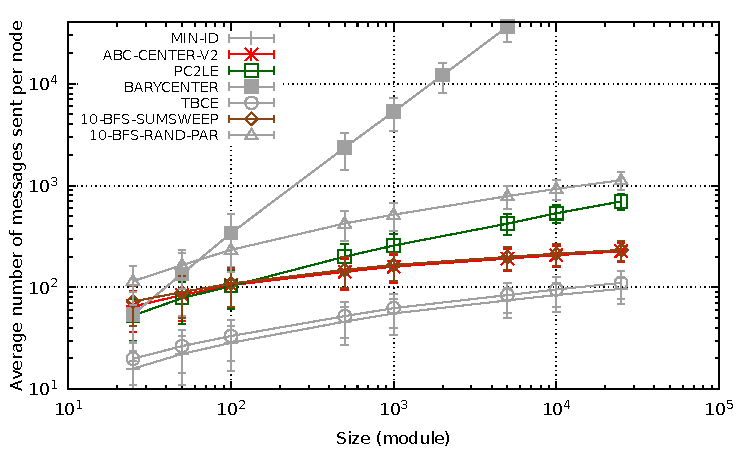
\includegraphics[width=0.9\linewidth]{fig/centrality/avgMessages}
\end{center}

\remark{A good trade-off between cost and accuracy}
\end{frame}


\begin{frame} \frametitle{Memory usage}

\begin{figure}
	\centering
	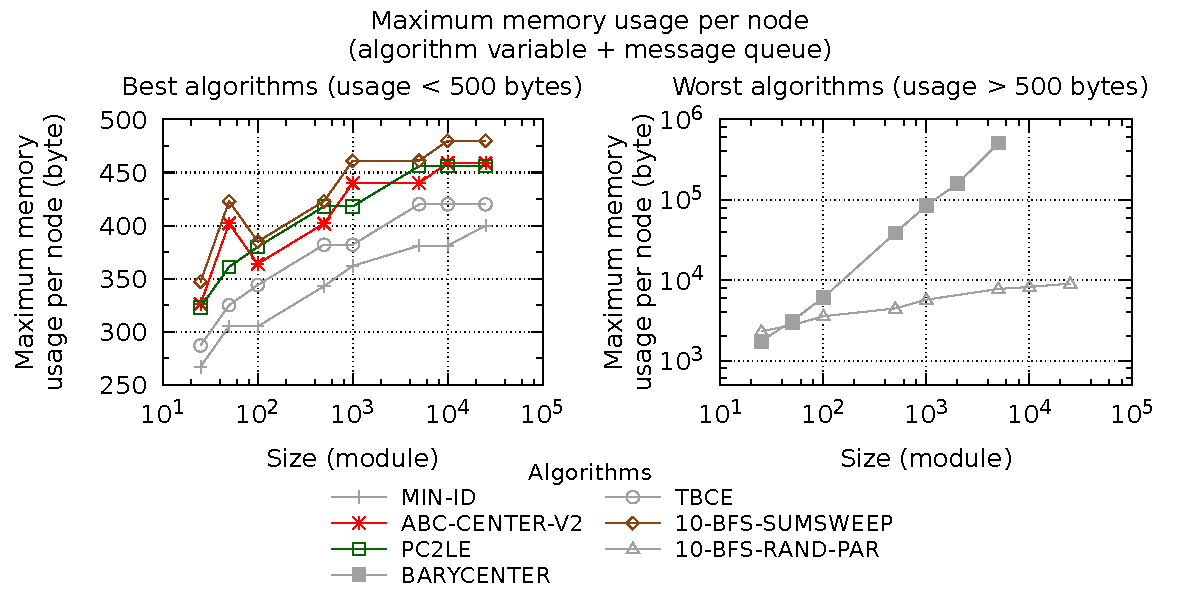
\includegraphics[width=0.9\linewidth]{fig/centrality/memory-defense}
\end{figure}

\remark{Our algorithms have a bounded and limited memory usage\\($< 500$ bytes per module)}

\end{frame}

\subsection{Conclusion}

\begin{frame} \frametitle{Conclusion}

\begin{itemize}
	\item 3 efficient distributed centrality-based leader election algorithms
		\begin{itemize}
			\item $k$-BFS SumSweep, ABC-Center and PC2LE
		\end{itemize}
	\item Robustness to network dynamics
	\item Formal analysis of the performance (time, message and memory)
	\item Evaluation
		\begin{itemize}
			\item Hardware: 5 to 64 modules
			\item Simulations: 10 to 25,000 modules
			\begin{itemize}
				\item Most precise approximation algorithms ($> 85\%$ relative center accuracy)
				\item Good cost-accuracy trade-off 
			\end{itemize}
		\end{itemize}
	\item Limits
		\begin{itemize}
			\item Experimental evaluation of the accuracy
			\item Bad cases?
			\item Efficiency in other platforms with different network structures?
				\begin{itemize}
					\item Our algorithms: inspired from external-graph analysis algorithms used to study large-scale real-world networks (e.g., YahooWeb, AS networks)
				\end{itemize}
		\end{itemize}
\end{itemize}
\end{frame}